\documentclass[10pt]{article}
\usepackage[margin=0.8in]{geometry}
\usepackage{graphicx,amsmath,hyperref}
\setlength{\parindent}{0pt}
\setlength{\parskip}{7pt}
\begin{document}
\begin{center}
{\Large Guarded fall degrees: Lean proof progress}\\
2026-10-29 --- Exact-pair target remains open
\end{center}

The requested theorem is the exact ordinary first/last fall pair $(4,5)$ for
every unsatisfiable inverse-guarded three-abscissa short-Weierstrass system
under the study's rational-point and characteristic hypotheses.

\textbf{New verified theorem.} For every field $K$ with $6\ne0$, every three
distinct $a,b,c\in K$, and arbitrary curve coefficients and target abscissa,
\texttt{GuardedModel.no\_degree\_four\_refutation} proves
$1\notin V(F,4)$ for the actual six generators. It uses neither recorded
ranks nor a hypothesis asserting the lower bound. With an explicit unit-ideal
hypothesis, \texttt{lastFall\_lower} excludes all last-fall bounds below five.
The field-of-definition/unit-ideal bridge is still open.

\textbf{Structural proof.} Ordinary closure is defined on Mathlib multivariate
polynomials by finite derivations, including arbitrary multipliers when the
actual product has degree within the bound. Its least-subspace property and
the last-fall/refutation equivalence for unit ideals are checked. The
separating space is $I+Kf_1+Kf_2$, where $I$ vanishes on the guarded base
grid while $u$ remains formal. Its degree-at-most-three part lies in $I$:
the affine $u^2$ coefficient cannot interpolate nonzero quartic weights on
three distinct points. Degree additivity proves full multiplicative closure
at four. The space excludes one by grid evaluation.

\begin{center}
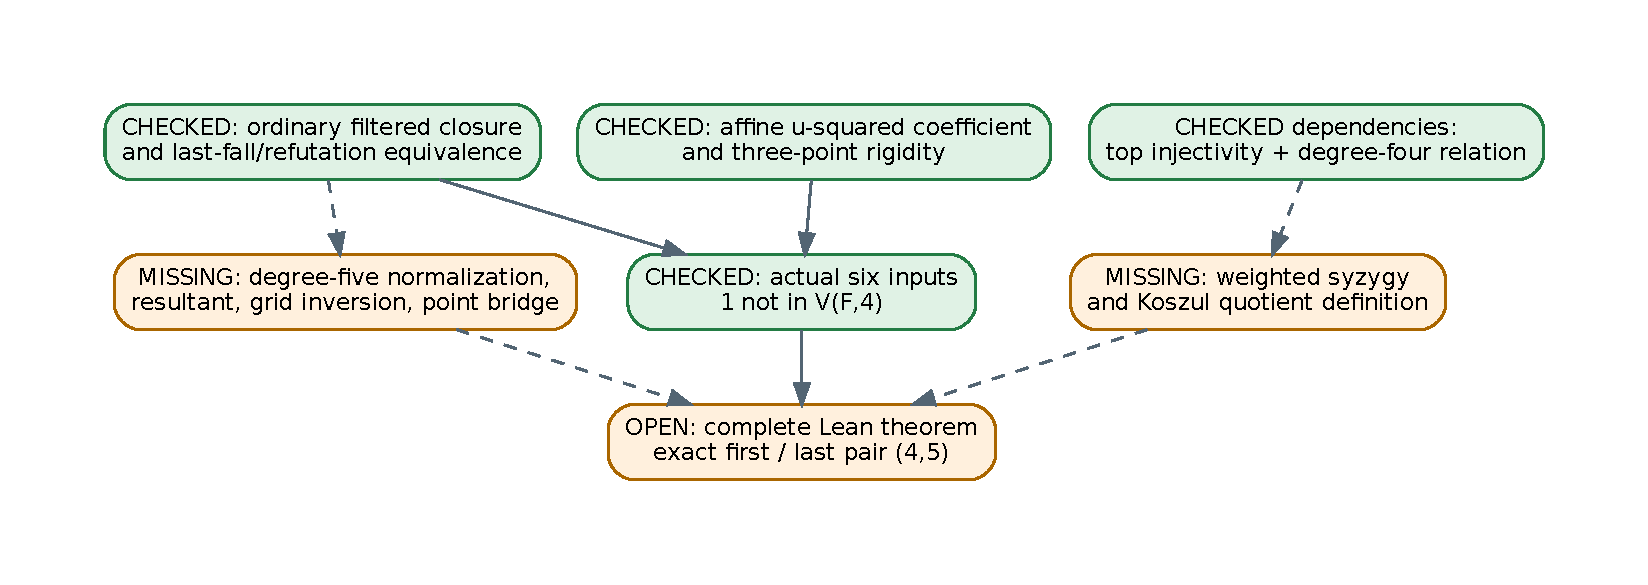
\includegraphics[width=0.96\linewidth,height=0.43\textheight,keepaspectratio]{exact-pair-coverage.pdf}
\end{center}

\textbf{Additional checked dependencies.} The quadratic divided difference
is actually derived inside $V(F,4)$ with polynomial degree bounds.
Low-degree top-map injectivity, the degree-four homogeneous relation and its
lift are checked. A weighted syzygy/Koszul formalization is still required
before claiming the numeric first-fall equality.

\textbf{Reproduce.} Pinned Lean 4.34.1, Mathlib
\texttt{d13f23b723b8a846827a245b89c10fc7d3f11612}.
Run \texttt{lake build}, the repository's \texttt{AuditAxioms.lean} on all six
new modules, and fresh \texttt{leanchecker} on \texttt{FirstFallCore}.
Exact commands, logs, hashes and hypotheses are in
\texttt{exact-pair-progress.md} and \texttt{exact-pair-validation/}.
Only standard Lean foundations are accepted; no custom theorem axioms,
compiler-trusting evaluation or placeholders are used.

\textbf{Remaining scope.} The universal degree-five normalization,
resultant, finite-grid inversion and rational-point bridge are not yet
formalized. Thus the requested exact pair is partial. No new experiments,
timings, growing-base or characteristic-two degree claims are made.
Sources: Huang--Kosters--Yang--Yeo, arXiv:1505.02532, Definitions 2.1--2.2;
the study's symbolic and independent audits; pinned Mathlib sources.
\end{document}
